\documentclass[11pt]{article}

% load some asm stuff -
\usepackage{amssymb}
\usepackage{amsmath}
\usepackage{amsthm}
%\usepackage{palatino,lettrine}
\usepackage{fancyhdr}
\usepackage{epsfig}
\usepackage[round,comma,sort]{natbib}
\usepackage{simplemargins}
\usepackage{setspace}
\usepackage{wrapfig}
\usepackage{hyperref}
%\usepackage{boiboites}
\usepackage[margin=0pt,font=small,labelfont=bf]{caption}
\newcommand{\boldindex}[1]{\textbf{\hyperpage{#1}}}
\usepackage{makeidx}\makeindex
\bibliographystyle{plos2015}


\usepackage{algpseudocode}
\usepackage{algorithm}

% Set the size
%\textwidth = 6.75 in
%\textheight = 9.75 in
%\oddsidemargin = 0.0 in
%\evensidemargin = 0.0 in
%\topmargin = 0.01 in
%\headheight = 0.0 in
%\headsep = 0.25 in
%\parskip = 0.15in
% \doublespace
\setallmargins{1in}

\newtheorem{example}{Example}[section]
\newtheorem{thm}{Theorem}[section]
\newtheorem{property}{Property}[section]

\theoremstyle{definition}
\newtheorem{defn}[thm]{Definition}

\makeatletter
% \renewcommand\subsection{\@startsection
% 	{subsection}{2}{0mm}
% 	{-0.05in}
% 	{0.1\baselineskip}
% 	{\normalfont\normalsize\bfseries}}
\renewcommand\subsubsection{\@startsection
	{subsubsection}{2}{0mm}
	{-0.05in}
	{-0.5\baselineskip}
	{\normalfont\normalsize\itshape\bfseries}}
\renewcommand\paragraph{\@startsection
	{paragraph}{2}{0mm}
	{-0.05in}
	{-0.5\baselineskip}
	{\normalfont\normalsize\itshape}}
\makeatother
\linespread{1.1}

\fancypagestyle{proposal}{\fancyhf{}%
	\fancyhead[RO,LE]{\thepage}%
	\fancyhead[LO,RE]{CHEME 131 Module 1 Zero Coupon Treasury Securities}%
	\renewcommand\headrulewidth{1pt}}
\pagestyle{proposal}

\usepackage{mdframed}
\definecolor{lgray}{rgb}{0.92,0.92,0.92}
\definecolor{antiquewhite}{rgb}{0.98,0.92,0.84}
\definecolor{lightskyblue}{rgb}{0.93,0.95,0.99}

% defn environment
\mdfdefinestyle{theoremstyle}{% 
    linecolor=black,linewidth=1pt,% 
    frametitlerule=true,% 
    frametitlebackgroundcolor=lgray, 
    innertopmargin=\topskip,} 
\mdtheorem[style=theoremstyle]{definition}{Definition}

% concept environment
\mdfdefinestyle{conceptstyle}{% 
    linecolor=black,linewidth=1pt,% 
    frametitlerule=true,% 
    frametitlebackgroundcolor=lightskyblue, 
    innertopmargin=\topskip,} 
\mdtheorem[style=conceptstyle]{concept}{Concept}
\newcommand{\newterm}[1]{{\it #1}}

% Single space'd bib -
\setlength\bibsep{0pt}

\renewcommand{\rmdefault}{phv}\renewcommand{\sfdefault}{phv}
%\newboxedtheorem[boxcolor=black, background=gray!5,titlebackground=orange!20,titleboxcolor = black]{color_box_example}{Example}{test}

% Change the number format in the ref list -
\renewcommand{\bibnumfmt}[1]{#1.}

% Change Figure to Fig.
\renewcommand{\figurename}{Fig.}
\usepackage{enumitem}
\setlist{noitemsep} % or \setlist{noitemsep} to leave space around whole list

%Joycelyn Chan, Joshua Lequieu, Michael Paull, Chidanand Balaji, Ryan Tasseff
%Our derivation follows closely the earlier development of Fredrickson \citep{Fredrickson:1976fk}.

% Begin ...
\begin{document}

%\begin{titlepage}
{\par\centering\textbf{\Large CHEME 131 Module 1: Abstract Assets and the Pricing of Zero Coupon Treasury Securities}}
\vspace{0.2in}
{\par \centering \large{Jeffrey D. Varner}}
\vspace{0.05in}
{\par \centering \large{Smith School of Chemical and Biomolecular Engineering}}
{\par \centering \large{Cornell University, Ithaca NY 14853}}
% \vspace{0.1in}
% {\par \centering \small{Copyright \copyright\ Jeffrey Varner 2018. All Rights Reserved.}}\\

%\end{titlepage}
\date{}
\thispagestyle{empty}

\setcounter{page}{1}

% \begin{mdframed}[backgroundcolor=lgray]

% 	\subsection*{Background}
% 	We have discussed idealized reversible power generation and refrigeration cycles, and considered the impact of
% 	process irreversibility. In this lecture module, we will expand on the topic of irreversibility. In particular, we will develop expressions for
% 	the rate of \textit{lost work} caused by irreversibility in terms if the rate of entropy generation and process unit efficiencies.

% 	\vspace{0.1in}
% 	\subsection*{Student outcomes}
% 	At the end of this lecture module, students will be able to:
% 	\begin{itemize}
% 	  \item[O$_1$]{Describe the terms in the entropy balance for an open time dependent and steady-state system}
% 		\item[O$_2$]{Relate the rate of lost work $\dot{W}_{lost}$ to the rate of entropy generation $\dot{S}_{G}$ in a steady-state system.}
% 		\item[O$_3$]{Relate the efficiency of common equipment, e.g., pumps, compressors turbines etc to the rate of entropy generation $\dot{S}_{G}$ in a steady-state system.}
% 	\end{itemize}

% \end{mdframed}

% \clearpage

\section*{Introduction}
\href{https://www.investor.gov/introduction-investing/investing-basics/glossary/treasury-securities}{United States Marketable Treasury Securities}, 
are issued by the U.S. Department of the Treasury to fund its operations and meet financial obligations. 
These debt securities are structured loan agreements between a borrower, i.e., the U.S. government, and a lender (you) 
that allows the government to fund its operations and obligations (Fig. \ref{fig:govt-debt-schematic}).
The debt holder and the U.S. Treasury have a marketable repayment agreement, which can be held by the lender (you) until the completion of the contract or resold on a secondary market. Although there are various types of U.S. government debt securities, they all share a few common characteristics. 
First, U.S. Treasury debt securities have a predetermined term length; thus, the contract duration between the borrower and lender is fixed.
Second, U.S. Treasury debt securities have a par value, representing the instrument's face value, a price (which may differ from the par value), and an interest rate paid to the lender. Next, some U.S. Treasury debt securities have interest payments commonly called coupons. These payments give the lender fixed cashflows on a predetermined schedule throughout the debt instrument's term. Finally, income from interest on U.S. Treasury debt securities is free of state and local income taxes but subject to federal income taxes.
You can purchase U.S. Treasury debt directly from the \href{https://www.treasurydirect.gov/indiv/products/prod_tbonds_glance.htm}{United States Treasury via TreasuryDirect} 
or through a bank or broker to lend money to the U.S. government.

\begin{figure}[h]
    \centering
    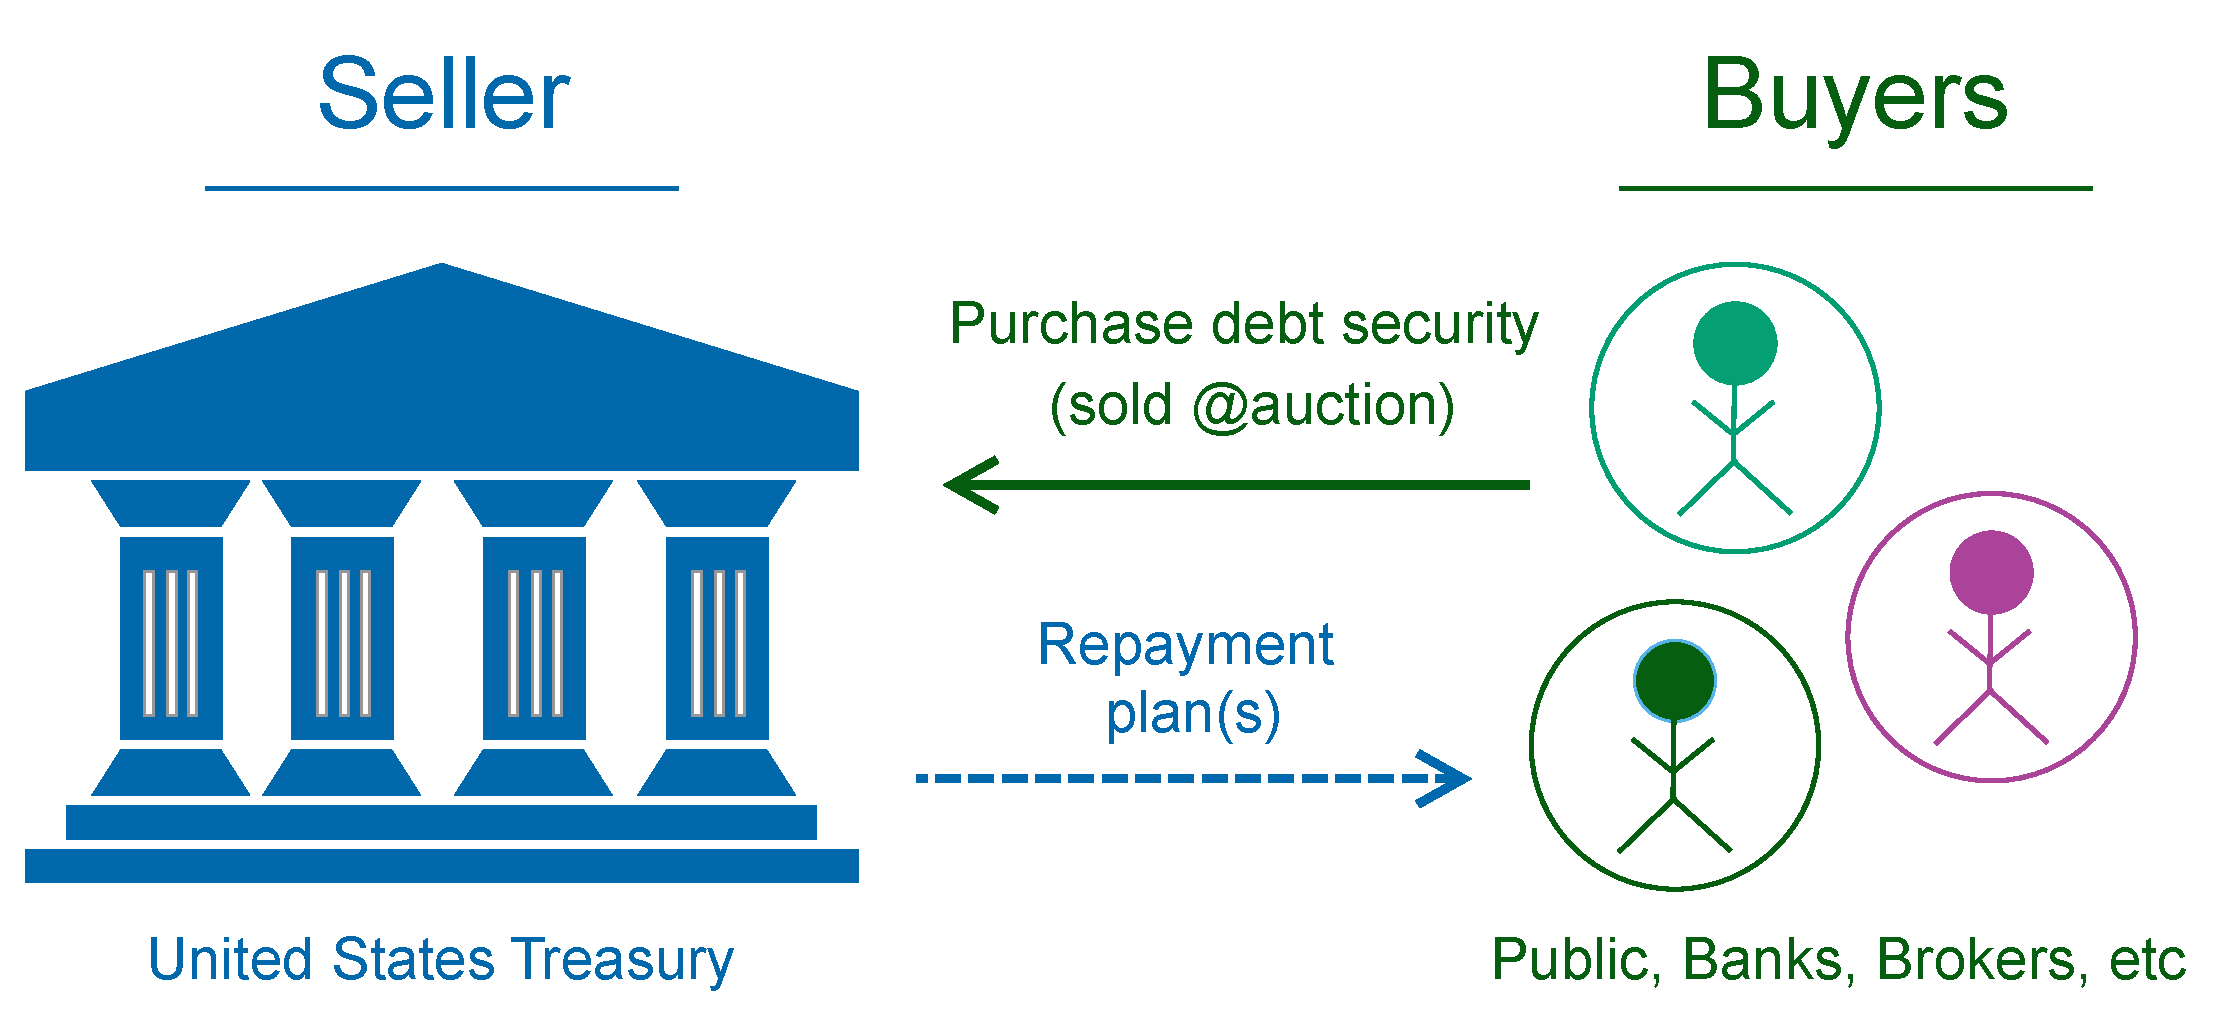
\includegraphics[width=0.85\textwidth]{./figs/Fig-Govt-Debt-Schematic.pdf}
    \caption{Schematic of U.S. Government Debt Securities. }\label{fig:govt-debt-schematic}
\end{figure}

\section*{Prerequisites}
Throughout all the courses we'll make use of a few concepts and approaches from finance, mathematics, statistics, and computer science.
Let's begin this module by reviewing some of these concepts, in particular the concept of an abstract asset and the time value of money.
These two foundational concepts are essential for understanding the pricing of zero-coupon Treasury securities (and other financial instruments).
They also provide a useful framework for financial decision-making.

\subsection*{Abstract Assets}
The traditional view of an \href{https://en.wikipedia.org/wiki/Asset}{asset} is perhaps a physical resource with economic value that an individual, corporation, or country owns or controls with the expectation that it will provide a future benefit.
For example, a car, house, or piece of land are all assets.
However, in a more general sense, we can also think of an asset as a sequence of current and future cash flows demarcated in some currency, for example, Euros, Dollars, Yuan, or cryptocurrencies such as Bitcoin.
This more genetral notiion of an asset, which we'll refer to as an \newterm{abstract asset}\index{Abstract asset}, is a useful mental model for thinking about the pricing of financial instruments, e.g., stocks, bonds, and derivatives, 
as well as the valuation of projects and other investments, and even traditional physical assets.
In this model, cash flows can be positive or negative, and assets can be tangible or intangible.
The challenge with this framework is that current and future cash flows are not directly comparable,
i.e., we cannot add or subtract a cash flow that occurs today, with a cash flow that occurs at a different time in the future.
We can think of these cash flows as being in different currencies, e.g., dollars versus euros, that must be exchanged. 
Thus, we formulate the equivalent of an exchange rate to compare cash from different periods.
This is the concept of the time value of money, discount factors, and discount rates which we discuss next.

\subsection*{Time Value of Money}
At firts glance, the idea that money has a time value seems counterintuitive. 
If I put a dollar in my pocket today, it is still a dollar tomorrow, next week, or next year. 
However, the value of a dollar today, e.g., the Utility that it brings  to you by purchasing a good or serice is not the same as the value of a dollar tomorrow.
The change in the value of money over time is called the time value of money (Concept \ref{concept:time-value-of-money}):
\begin{concept}[Time value of money]\label{concept:time-value-of-money}
	One dollar today is not worth the same as one dollar tomorrow. 
	The change in the value of money over time is called the \newterm{time value of money}\index{The time value of money}.
\end{concept}
The time value of money is an empirical observation that has been seen over hundreds of years. 
But why is this the case? Short answer: Money given to us today has a greater \href{https://en.wikipedia.org/wiki/Utility}{Utility} 
than the same amount tomorrow because we have an extra day to invest (or use) that money. Suppose a \emph{risk-free} investment is guaranteed to return an interest rate of $i>0$ per period.
If we invested $P$ dollars today in this risk-free investment, at the end of the investment period, e.g., a day, week, year, etc., 
we are \emph{guaranteed} to get $F$ dollars back (because the investment is risk-free):
\begin{equation*}
F = (1+i)\cdot{P}
\end{equation*}
where $F$ is the future value of the investment, $P$ is the present value of the investment, and $i$ is the interest rate per period.
Thus, if given a choice between $P$ dollars today or $P$ dollars one investment period in the future, 
a rational investor would always choose to take the $P$ dollars now. By taking $P$ dollars today, you could invest those $P$ dollars risk-free and get $F = (1+i)\cdot{P}$ back, where $F>P$. 
In this hypothetical world, the only case where it makes sense to take the future money is if $i\leq{0}$, i.e., $F\leq{P}$, which is forbidden by the condition $i>0$. 
This hypothetical scenario assumes that a risk-free investment exists that always returns an interest rate of $i>0$; 
does such an investment exist? 

\href{https://www.investopedia.com/terms/r/risk-freerate.asp}{Unfortunately, an actual risk-free investment is only a theoretical concept}. 
However, the risk-free rate of return $i$ is often approximated by the yield on US Treasury debt securities because US Treasury debt securities are backed by the full faith and credit of the United States government
and are considered one of the safest investments in the world. 
Thus, we can use the yield on US Treasury debt securities as a proxy for the risk-free rate of return $i$. 
This is the first reason why we are interested in these securities.

\subsubsection*{Exchange rate model.}
Now that we have established money’s present value is higher than its future value, we need a way to compare cash from different periods. 
A useful mental model for the time value of money is to think of money from different periods 
as being in other currencies (e.g., dollars versus euros) that must be exchanged. 
Thus, we can formulate the equivalent of an exchange rate to compare money or cash flows from different periods. 
For example, suppose we have an active asset over multiple periods, e.g., a multi-period project or some other transaction that occurs over many periods. 
Further, suppose we have a cash flow $\dot{c}_{t}$ in period $t$ that we want to convert to a cash flow $\dot{c}_{0}$ in period zero, e.g., the future sale of shares of stock.
In this case, we develop a multi-period conversion easily constructed by sequentially applying many one-period calculations. 
To see this idea, let's start with period zero to period one:
\begin{equation}\label{eq:period-zero-to-one}
\dot{c}_{1} = \left(1+r_{10}\right)\cdot\dot{c}_{0}
\end{equation}
where $r_{10}$ is the exchange rate (what we'll later call the \texttt{short rate}) from period zero to period one, and $\dot{c}_{0}$ is the cash flow in period zero.
Then, period one to period two is given by:
\begin{equation}\label{eq:period-one-to-two}
\dot{c}_{2} = \left(1+r_{21}\right)\cdot\dot{c}_{1}
\end{equation}
where $r_{21}$ is the exchange rate from period one to period two, and $\dot{c}_{1}$ is the cash flow in period one. 
However, we can substitute $\dot{c}_{1}$ from Equation \ref{eq:period-zero-to-one} into Equation \ref{eq:period-one-to-two} to give:
\begin{equation}\label{eq:period-one-to-two-substituted}
\dot{c}_{2} = \Bigl[\left(1+r_{21}\right)\left(1+r_{10}\right)\Bigr]\cdot\dot{c}_{0}
\end{equation}
If we do this computation between 2 and 3, and then 3 to 4, etc, we develop a relationship between the initial value of cash flow 
$\dot{c}_{0}$ and future $\dot{c}_{t}$ cash flow values (Defn. \ref{defn:multiple-period-discrete-conversion}):

\begin{definition}[Multiple period-dependent discrete discount]\label{defn:multiple-period-discrete-conversion}
Let $\dot{c}_0$ be the present cash flow, and $\dot{c}_t$ be the future cash flow in period $t$. 
Further, let $r_{j+1,j}$ represent the discount rate between discrete periods $j$ and $j+1$. Then: 
\begin{equation}
\dot{c}_{t} = \left[\prod_{j=0}^{t-1}\left(1+r_{j+1,j}\right)\right]\cdot\dot{c}_{0}\qquad{t=1,2,\dots,T}
\end{equation}
The term in the brackets is the \textit{multi-period discrete discount factor}, which we represent as the function $\mathcal{D}_{t,0}(r)$.
\end{definition}

Of course, an obvious challenge with this approach is that we need to know the discount rate(s) $r_{j+1,j}$ between every period $j$ and $j+1$.
In practice, this is not possible. However, supposewe  approximated the discount rate(s) $r_{j+1,j}$ with an effective rate $\bar{r}$ 
that was constant over the lifetime of the project or investment such that:
\begin{equation}\label{eq:effective-rate}
\left(1+\bar{r}\right)^{t} = \prod_{j=0}^{t-1}\left(1+r_{j+1,j}\right)
\end{equation}
Then, we can rewrite the multi-period discrete discount factor as:
\begin{equation}\label{eq:multi-period-discrete-discount-factor}
\mathcal{D}_{t,0}(\bar{r}) = \left(1+\bar{r}\right)^{t}
\end{equation}
where $\bar{r}$ is the effective discount rate. Finally, imagine the we have $\lambda$ compounding periods per year, 
and the effective discount rate $\bar{r}$ is an annualized rate (which is typically the case). 
Then we can rewrite the effective discount rate as:
\begin{equation}\label{eq:effective-rate-compounded}
\mathcal{D}_{t,0}(\bar{r}) = \left(1+\frac{\bar{r}}{\lambda}\right)^{\lambda\cdot{t}}
\end{equation}
where $\bar{r}$ is the discount rate, and $\lambda$ is the number of discounting events per period
(Defn. \ref{defn:multiple-effective-period-discrete-conversion}).
\begin{definition}[Multiple period effective discrete discount]\label{defn:multiple-effective-period-discrete-conversion}
	Let $\dot{c}_0$ be the present cash flow, and $\dot{c}_t$ be the future cash flow in period $t$. 
	Further, let $\bar{r}$ represent the (constant) effective discount rate, $\lambda$ is the number of discounting events per period. 
	Then:
	\begin{equation}
	\dot{c}_{t} = \left[\left(1+\frac{\bar{r}}{\lambda}\right)^{\lambda\cdot{t}}\right]\cdot\dot{c}_{0}\qquad{t=1,2,\dots,T}
	\end{equation}
	The term in the brackets is the \textit{multi-period effective discrete discount factor}, which we represent as the function $\mathcal{D}_{t,0}(\bar{r})$.
\end{definition}

\subsubsection*{A different perspective.}
In the exchange rate model, we converted cash flows from the future to the present (and vice-versa) using a period-dependent discount rate $r_{t+1,t}$, 
or an effective discount rate $\bar{r}$, and a discount factor $\mathcal{D}_{t,0}(r)$. These acted like exchange rates between different currencies.
However, this approach is often seen as confusing. For example, its not clear what discount rate to use, what a discount factor actually means practically, etc.
Toward this challenge, let's introduce a different perspective of discounting, and the discount rate.
Suppose we think of the discount rate $r_{t+1,t}$  (or $\bar{r}$) as the minimum 
\newterm{rate of return}\index{rate of return} that a decision-maker 
would accept for a project or investment. In this context, discount rates are like interest rates, that we can earn on an investment.
Let's continue with this idea and introduce the concept of interest, and interest rates.

There are two types of interest, simple and compound. The distinction between simple and compound interest is crucial in the world of finance and investing.
These concepts significantly impact investment growth and borrowing costs, making them fundamental aspects to consider when making financial decisions. 
Simple interest is paid only on the initial principle. 
For example, if amount $A(0)$ is invested in an account at $t=0$ which pays a simple interest rate of $r$ per period, 
then after $n$ periods the account will hold amount $A(n)$ (assuming no withdrawals, etc):
\begin{equation}\label{eq:simple-interest}
A(n) = A(0)\cdot\left(1+rn\right)
\end{equation}
On the other hand, compound interest considers both the principal and the interest accumulated over time. 
For example, if amount $A(0)$ is invested in an account at $t=0$ which pays a compound interest rate $r$ per period, 
then after $n$ periods the account will hold amount $A(n)$ (assuming no withdrawals, etc):
\begin{equation}\label{eq:compound-interest}
A(n) = A(0)\cdot\left(1+r\right)^n
\end{equation}
If there are multiple compounding periods per year, then the interest rate $r$ is divided by the number of compounding periods per year $\lambda$
and we arrive at the following expression for compound interest:
\begin{equation}\label{eq:compound-interest-multiple}
A(n) = A(0)\cdot\left(1+\frac{r}{\lambda}\right)^{n\cdot\lambda}
\end{equation}
Clearly, compound interest is more advantageous to the investor than simple interest. 
Furhtermore, Eqn. \eqref{eq:compound-interest-multiple} is equivalent to Defn. \ref{defn:multiple-effective-period-discrete-conversion}
when the interest rate $r$ is the effective discount rate $\bar{r}$, and the number of compounding periods per year $\lambda$ is the number of discounting events per period.
Finally, consider the case when the number of compounding periods per year $\lambda\rightarrow\infty$, i.e., we have continuous compounding (Defn. \ref{defn:continuous-compounding}):
\begin{definition}[Continuous compounding]\label{defn:continuous-compounding}
Let there be n-compounding periods per period, e.g., year and an annualized interest rate of $r$.  
Then an initial investment $A(0)$ will be worth:
\begin{equation}\label{eqn-compound-interest-model-discrete}
A(m) = A(0)\cdot\left(1+r/n\right)^{mn}
\end{equation}
after m-periods, e.g., m-years. As the number of compounding periods $n\rightarrow\infty$, 
the investment $A(m)$ approaches the continuous compounding limit:
\begin{equation}\label{eqn-compound-interest-model-cont}    
\lim_{n\rightarrow\infty}A(m) = A(0)\cdot\exp\left(rm\right)
\end{equation}
The quantity $\exp\left(rm\right)$ is the \textit{continuous compounding (discount) factor}, 
which we also represent (with a slight abuse of notiion) as $\mathcal{D}_{m,0}(r)$.
\end{definition}

\subsection*{Net Present Value (NPV)}
Now that we have tools to account for the time value of money, we can return to the question of how to value an asset. 
The most intuitive approach is to compute the net cash flow at every time point. Imagine at node $t=k$ we have $\mathcal{S}^{t=k}$ cash streams,
denoted as $\dot{c}_{s}$, entering (or exiting) the asset node. 
Then, the net cash flow at node $t=k$ is given by:
\begin{equation}\label{eq:net-cash-flow}
\bar{c}_{k} = \sum_{s\in\mathcal{S}^{t=k}}\nu_{s}\dot{c}_{s}
\end{equation}
where $\nu_{s}$ is a direction parameter; $\nu_{s}=+1$ if stream $s$ enters node $t=k$, $\nu_{s}=-1$ if stream $s$ exists node $t=k$. 
Finally, we sum all the current and future cash flows, converted to some shared basis, e.g., current dollars. 
This sum is called the Net Present Value (NPV); NPV is a widespread method for asset valuation and financial decision-making 
(Defn. \ref{defn:net-present-value}): 
\begin{definition}[Net Present Value (NPV)]\label{defn:net-present-value}
Let $\bar{c}_{t}$ be the net cash flow in period $t$. 
Then, the net present value (NPV) is the sum of current and future discounted cash flows:
\begin{equation}    
\text{NPV}(T,r) = \sum_{i=0}^{T}{\mathcal{D}_{i,0}^{-1}}(r)\cdot\bar{c}_{i}\qquad{T\geq{0}}
\end{equation}
where the term \texttt{T} is the number of time periods 
(lifetime of the project or investment), and $\mathcal{D}_{i,0}(r)$ is the multistep discount factor with discount rate(s) \texttt{r}
between period $i$ and period $0$.
\begin{itemize}[leftmargin=*]
\item{The discount factor $\mathcal{D}_{i,0}(r)$ can be either a discrete or a continuous discounting model.}
\item{The NPV does not require that the discount rate is constant over the lifetime of the project or investment, but this is often assumed.}
\item{The discount  $\mathcal{D}_{0,0}(r) = 1$ for all values of $r$.}
\end{itemize}
\end{definition}
The net present value (NPV) is a useful metric for financial decision-making.
In this context, the NPV has the following interpretations:
\begin{itemize}[leftmargin=*]
\item{$\textbf{NPV}<0$:~}{A negative NPV indicates the proposed project will generate less income than a hypothetical alternative investment, e.g., a risk-free investment at the same discount rate and time-to-maturity as the project.}
\item{$\textbf{NPV}=0$:~}{A zero NPV indicates the proposed project will generate the same income as a hypothetical alternative investment, e.g., a zero-coupon bond at the same discount rate and time-to-maturity as the project. }
\item{$\textbf{NPV}>0$:~}{A positive NPV indicates the proposed project will generate more income than a hypothetical alternative investment, e.g., a zero-coupon bond at the same discount rate and time-to-maturity as the project.}
\end{itemize}
The connection of the net present value (NPV) to the time value of money is clear.
However, the connection of the NPV with a zero-coupon bond is not. 
As we will see, the NPV of a project or investment with a zero NPV is equivalent to the price of a zero-coupon bond with the same time-to-maturity 
and discount rate. Thus, a rational investor would be indifferent between investing in a NPV = 0 project or investing in a zero-coupon bond.

\section*{Zero-Coupon Treasury Bills}\label{sec:treasury-bills}
Finally, let's focus on our first example of a U.S. Treasury security, the \href{https://treasurydirect.gov/marketable-securities/treasury-bills/}{Treasury Bill}.
\href{https://treasurydirect.gov/marketable-securities/treasury-bills/}{United States Treasury Bills}, \texttt{T-bills} or just \texttt{Zeros} are Treasury debt instruments with short-term maturity periods T = 4, 8, 13, 26, and 52 weeks 
and zero coupon payments, i.e., no seperate semiannual interest payments to the lender (you).
In the context of the abstract asset framework, T-bills have two cashflow events, namely when the lender (you) buys the T-bill at auction 
and when the borrower (United States Treasury) pays the lender (you) the face (par) value of the T-bill at maturity (Fig. \ref{fig:t-bill-schematic}).
\begin{figure}[h]
    \centering
    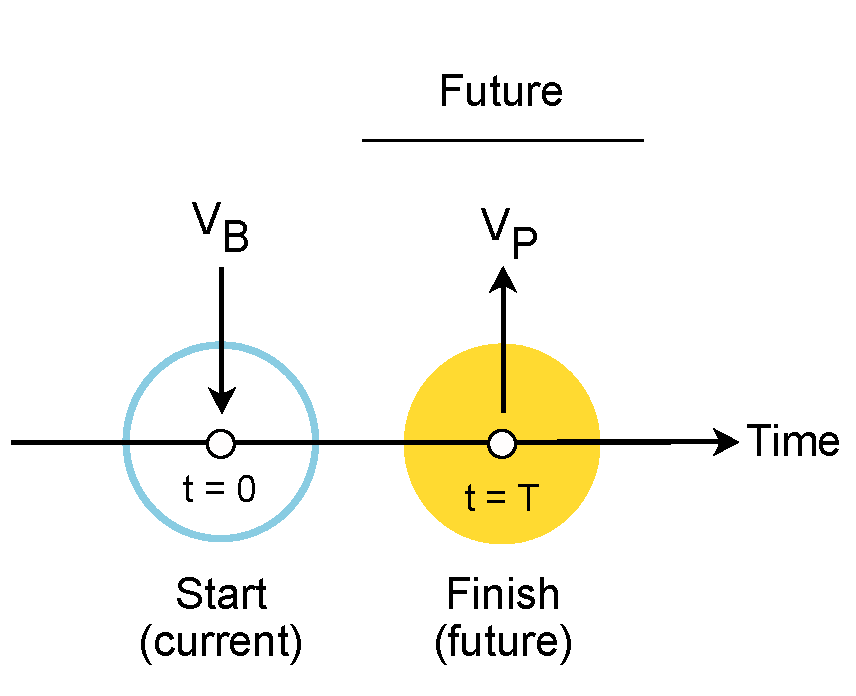
\includegraphics[width=0.5\textwidth]{./figs/Fig-Bill-Asset-Timeline-Schematic.pdf}
    \caption{Asbtract asset schematic of a zero-coupon Treasury bill. The lender (you) gives the United States Treasury 
    the price $V_{B}$ of the T-bill at auction at $ t = 0$. In return, the Treasury pays the bill holder (you) the par value of the T-bill $V_{P}$ at maturity $t>0$. 
	The schematic is written from the perspective of the borrower (United States Treasury).}\label{fig:t-bill-schematic}
\end{figure}
The price of a zero-coupon Treasury bill $V_{B}$ with an effective (constant) interest (discount) rate of $\bar{r}$ and a maturity of \texttt{T}-years at auction 
is the discounted face (par) value $V_{P}$ such that the net present value (NPV) of the bill is zero:
\begin{equation}    
\text{NPV}(T,\bar{r}) = -V_{B} + \mathcal{D}_{T,0}^{-1}(\bar{r})\cdot{V_{P}} = 0
\end{equation}
or equivalently:
\begin{equation}
    V_{B} = \mathcal{D}_{T,0}^{-1}(\bar{r})\cdot{V_{P}}
\end{equation}
The quantity \texttt{T} denotes the duration of the bill (in years), 
$\bar{r}$ is the effective annualized interest rate,  and $\mathcal{D}_{T,0}^{-1}(\bar{r})$ is the inverse multistep discount factor
for period $0\rightarrow{T}$. 
Theorectically, the discount factor $\mathcal{D}_{T,0}^{-1}(\bar{r})$ can be computed on either a discrete or continuous basis. 
However, in the case of treasury securities, the discount factor is computed on a discrete basis, assuming $\lambda$ compounding events per year, 
where typcially $\lambda = 2$, i.e., semi-annual compounding.


\clearpage
\printindex

\end{document}
